\documentclass[journal]{IEEEtran}
\ifCLASSINFOpdf
\else
\fi
\usepackage{times}
\usepackage{latexsym}
\usepackage{array}
\usepackage{float}
\usepackage{graphicx}
\usepackage{tabularx}
\usepackage{amssymb}
\usepackage{hyperref}
\hyphenation{op-tical net-works semi-conduc-tor}


\begin{document}
\title{Fluent and Cohesive: Sub-Second Voice Interaction with General-Purpose Open-Weight Models on a 20-Watt Edge Device}
%
%
% author names and IEEE memberships
% note positions of commas and nonbreaking spaces ( ~ ) LaTeX will not break
% a structure at a ~ so this keeps an author's name from being broken across
% two lines.
% use \thanks{} to gain access to the first footnote area
% a separate \thanks must be used for each paragraph as LaTeX2e's \thanks
% was not built to handle multiple paragraphs
%

\author{Shaw Tan,
        Claire Tan
}

% note the % following the last \IEEEmembership and also \thanks - 
% these prevent an unwanted space from occurring between the last author name
% and the end of the author line. i.e., if you had this:
% 
% \author{....lastname \thanks{...} \thanks{...} }
%                     ^------------^------------^----Do not want these spaces!
%
% a space would be appended to the last name and could cause every name on that
% line to be shifted left slightly. This is one of those "LaTeX things". For
% instance, "\textbf{A} \textbf{B}" will typeset as "A B" not "AB". To get
% "AB" then you have to do: "\textbf{A}\textbf{B}"
% \thanks is no different in this regard, so shield the last } of each \thanks
% that ends a line with a % and do not let a space in before the next \thanks.
% Spaces after \IEEEmembership other than the last one are OK (and needed) as
% you are supposed to have spaces between the names. For what it is worth,
% this is a minor point as most people would not even notice if the said evil
% space somehow managed to creep in.


% \markboth{Journal of \LaTeX\ Class Files,~Vol.~14, No.~8, August~2015}%
%{Shell \MakeLowercase{\textit{et al.}}: Bare Demo of IEEEtran.cls for IEEE Journals}




% If you want to put a publisher's ID mark on the page you can do it like
% this:
%\IEEEpubid{0000--0000/00\$00.00~\copyright~2015 IEEE}
% Remember, if you use this you must call \IEEEpubidadjcol in the second
% column for its text to clear the IEEEpubid mark.



% use for special paper notices
%\IEEEspecialpapernotice{(Invited Paper)}




% make the title area
\maketitle

% As a general rule, do not put math, special symbols or citations
% in the abstract or keywords.
\begin{abstract}
A voice assistant is fluent when its reply begins within the human turn-taking window — first audio in well under a second — and cohesive when the thing replying is a full large language model rather than an intent router. Production voice AI today gets one or the other: datacenter cascades median 1.4–1.7 s to first audio \cite{sharma2026latency,hamming2026metrics}, and the systems that beat the window do it with purpose-trained speech-to-speech models (Moshi \cite{defossez2024moshi}) that give up the text LLM's generality. We show both are achievable at the same time, entirely on a 20 W, credit-card-sized edge board, using unmodified state-of-the-art open-weight models.

Our pipeline — streaming ASR (whisper.cpp), a Gemma 4 model (2B–12B) on a purpose-built $\sim$6,000-line C/CUDA runner, and a VITS TTS (piper) — reaches 0.65 s from end of speech to first audio on a Jetson Orin NX 16GB responding to a 30-second spoken instruction, with the entire stack holding 4.2 GB of unreclaimable memory (it fits an 8 GB Jetson Nano) and peaking near 20 W. Four techniques carry the result, none of which modify the models: (1) prefill under speech — streaming ASR commits prefill into the open turn while the user is still speaking, backed by a proof that space-boundary splits are exact for SentencePiece, cutting post-speech TTFT from 5.37 s to 0.55 s on the 12B; (2) the LLM as clause splitter — a system prompt that makes the model create TTS flush points, motivated by the measured finding that the baseline model emits 21-word sentences with zero commas, leaving a clause-flushing TTS layer nothing to flush; (3) a streaming vocoder from stock TTS voices — ONNX graph surgery splits piper's monolithic VITS at the latent boundary so the HiFi-GAN decoder (finite receptive field) runs in overlapped chunks, making first PCM O(1) in clause length (0.10 s vs 0.27–0.49 s), sample-exact against the monolithic decode; (4) multi-token-prediction speculative decoding characterized honestly as content-dependent (1.1–2.1×) and as a battery feature (2.29 vs 2.85 J/token). A cross-silicon study against Moshi on an RTX A5000 finds the remaining gap to speech-native models is structural (one decoded clause + one vocoder call, $\sim$0.2 s) — and that the datacenter GPU buys only 1.7× over the 20 W board, because in the conversational regime the pipeline is floor-bound, not compute-bound.
\end{abstract}

%\begin{IEEEkeywords}
%IEEE, IEEEtran, journal, \LaTeX, paper, template.
%\end{IEEEkeywords}






% For peer review papers, you can put extra information on the cover
% page as needed:
% \ifCLASSOPTIONpeerreview
% \begin{center} \bfseries EDICS Category: 3-BBND \end{center}
% \fi
%
% For peerreview papers, this IEEEtran command inserts a page break and
% creates the second title. It will be ignored for other modes.
\IEEEpeerreviewmaketitle



\section{Introduction}
% The very first letter is a 2 line initial drop letter followed
% by the rest of the first word in caps.
% 
% form to use if the first word consists of a single letter:
% \IEEEPARstart{A}{demo} file is ....
% 
% form to use if you need the single drop letter followed by
% normal text (unknown if ever used by the IEEE):
% \IEEEPARstart{A}{}demo file is ....
% 
% Some journals put the first two words in caps:
% \IEEEPARstart{T}{his demo} file is ....
% 
% Here we have the typical use of a "T" for an initial drop letter
% and "HIS" in caps to complete the first word.
\IEEEPARstart{C}{onversation}  has a clock. Human turn transitions cluster tightly around a near-zero modal gap, with a cross-linguistic mean of roughly 200 ms \cite{stivers2009turntaking}; beyond one second a reply reads as hesitation, and industry telemetry places the median production voice agent at 1.4–1.7 s with a P90 of 3.3–3.8 s (P95 4.3–5.4 s) — the region of talk-overs and user frustration \cite{sharma2026latency,hamming2026metrics}. We name the two properties this paper pursues:

    \begin{itemize}
        \item Fluent: time from end of user speech to the first audio sample of the reply (TTFB) under one second — inside or adjacent to the human window.
        \item Cohesive: the reply is produced by a state-of-the-art general-purpose LLM in the loop — capable of instruction following, world knowledge, multi-turn context, tool use, and (in the same family) vision — not a latency-optimized intent model.
    \end{itemize}

The two properties pull apart because of where each is cheap. Datacenter cascades are cohesive but pay network, queueing, and orchestration latency. Speech-native full-duplex models such as Moshi \cite{defossez2024moshi} are strikingly fluent — we measure $\sim$130 ms TTFB on an RTX A5000 — but are purpose-trained speech models (a $\sim$7B Helium backbone fused to a neural codec), trained once, at great cost, with the conversational behavior baked in: no drop-in model upgrades, no text-domain tooling, no camera feed.

This paper takes the third corner: a cascaded pipeline of unmodified open-weight components — whisper.cpp ears, Gemma 4 brain, piper mouth — on a Jetson Orin NX 16GB, chosen as the robotics-relevant operating point (the AGX steps up in both power and cost; the Nano 8GB lacks the RAM headroom for the larger family members, though Section V-F shows our smallest configuration fits it). All Gemma 4 family models produce cohesive conversation out of the box; the entire challenge is speed, and the paper is the anatomy of where the time goes and how it is reclaimed.

Contributions:

    \begin{enumerate}
        \item Prefill under speech (Section IV-B): incremental prefill of an open turn fed by streaming-ASR commit semantics, with a correctness lemma — SentencePiece pieces never cross a space boundary, so word-boundary splits reproduce the one-shot tokenization exactly (verified: equal token ids, byte-identical replies). A 929-token spoken instruction costs 0.55 s TTFT after the last word instead of 5.37 s (12B; 0.10 s on the 2B).
        \item The LLM as the clause splitter (Section IV-C): the split policy for streaming TTS must live in the model, because the measured baseline emits 21-word, comma-free sentences — there is nothing downstream to flush. A system prompt creates the flush points and cuts first audio from 1.21 s to 0.82 s; finetuning for human pause placement is the identified production path.
        \item A streaming vocoder from stock voices (Section IV-D): the published piper ONNX is monolithic, but exactly one tensor crosses into its HiFi-GAN decoder; automatic graph surgery splits any stock voice there — no retraining — and the decoder's finite receptive field makes overlapped-chunk decode sample-exact (max diff 4e-7, two voices, two machines). First PCM becomes O(1) in clause length: 0.10 s on the Orin where the monolithic call took 0.27–0.49 s. The full ablation ladder: first audio 1.21 → 0.82 (clause prompt) → 0.65 s (+streaming vocoder).
        \item A latency-anatomy protocol for local voice agents (Section IV-A): the decomposition TTFT → time-to-first-speakable → TTFB, measured client-side under three delivery modes (deferred / burst / paced-realtime), with warmup-discard and byte-identity discipline. TTFT alone is shown to be uninformative for the spoken experience.
        \item The whole-system result (Section V): 0.65 s TTFB on 20 W; three latency/ intelligence tiers from one runner (12B / E4B / E2B); 4.2 GB unreclaimable for ears+brain+mouth (8 GB-board feasible, with the measurement methodology that makes that number honest on Jetson); a decode rate that beats llama.cpp on the same board (1.17–1.26×) from $\sim$6,000 lines of C/CUDA.
        \item A cross-silicon study (Section V-H) against Moshi on its own class of hardware, locating the cascade's structural floor (one clause of decode + one VITS call) and showing the conversational regime is floor-bound: a datacenter GPU + desktop CPU improves end-to-end latency only 1.7× over the 20 W board.
    \end{enumerate}

\section{Related Work}

\textbf{Speech-native duplex models:} Moshi \cite{defossez2024moshi} fuses a 7B text backbone with the Mimi streaming codec and full-duplex dialogue training; the paper itself reports a theoretical latency of 160 ms, 200 ms in practice \cite{defossez2024moshi} (the reference implementation attributes this practical figure to an NVIDIA L4 — 24 GB, $\sim$72 W TDP datacenter card — a hardware detail from the project repository rather than the paper text \cite{kyutai2024moshirepo,nvidial4}); we measure $\sim$130 ms TTFB warm on an RTX A5000 (trials 252/129/135 ms; the $\sim$23 ms WebSocket handshake is excluded by construction — the clock starts when the client begins streaming audio, after the handshake byte). Two disclosures make this number conservative in Moshi's favor: our run used the uncompiled PyTorch q8 path (torch.compile is broken on Windows), and the clock anchors at the start of input streaming, measuring the full-duplex loop latency ($\sim$one 80 ms Mimi frame + one model step) rather than a turn response; Section VII discusses the anchor mismatch with our end-of-speech metric. Mini-Omni and its successor \cite{xie2024miniomni,xie2024miniomni2} follow the same species. These systems set the fluency bar, at the price of a fixed, purpose-trained model: the backbone is frozen into a speech topology, so the brain cannot be swapped for next quarter's better open-weight release, and text-ecosystem capabilities (tools, structured output, long instructions, vision) regress to what the speech training preserved.

\textbf{Cascaded voice pipelines:} Commercial stacks (Pipecat \cite{pipekit}, LiveKit Agents \cite{livekitagents}) cascade ASR → LLM → TTS and already stream at existing sentence punctuation. HuggingFace's speech-to-speech (v0.2.10 \cite{hfspeech2speech}) is the closest published relative — open-weight, modular, LLM over an OpenAI-compatible HTTP endpoint — and we benchmark it head-to-head on our board with our exact LLM (Section V-I). Our measurements locate the latencies these stacks leave on the table: prefill of the growing turn (hidden under speech, Section IV-B), the absence of early punctuation to flush on (created by the model itself, Section IV-C), and whole-sentence TTS synthesis before the first sample (Section IV-D).

\textbf{Local inference runtimes:} llama.cpp \cite{llamacpp} is the gold-standard general local runtime, and its throughput numbers are the reference we benchmark against (Section V-B). The pursuit of TTFB, however, is a different race than tokens/second: it rewards an appendable conversation abstraction (connection = conversation, line = turn, typed media/text frames into the open turn), speculative decoding tuned for short structured replies, and a server that streams the raw token channel for downstream clause flushing. little-gemma is not a llama.cpp competitor; it is a demonstration that a small, single-family runner can occupy a design point the general runtime does not: on the same Orin, matching $\sim$0.8× of llama.cpp's prefill while beating it 1.17–1.26× in decode, and — the relevant number for this paper — reaching first-sentence 18–48× earlier on multimodal turns (Section V-B, thought suppression and encode-off-critical-path).

\textbf{Streaming ASR:} whisper\_streaming / LocalAgreement-2 \cite{machacek2023whisper} provides the commit semantics our prefill rides on; the ASR side is prior art we consume, not a contribution.

\textbf{Speculative decoding:} EAGLE \cite{li2024eagle}, Medusa \cite{cai2024medusa}, self-speculation. Gemma 4 ships a first-party MTP head; our contribution is not the mechanism but the honest characterization (content- and head-width-dependence) and the energy angle (Section IV-E), which the edge literature largely lacks.

\section{System}
Hardware: Jetson Orin NX 16GB module (Ampere iGPU, shared LPDDR5), NVMe SSD, JetPack 6.2.1, headless. Rationale: the NX is the robotics operating point — credit-card footprint, 10–25 W envelope (40 W MAXN available), $\sim$\$600-class as a bare module (1KU pricing) or $\sim$\$900-class as a complete carrier-board dev kit \cite{arrow2026orin}. The AGX buys performance with a power/cost step that changes the product class; the Nano 8GB cannot hold the 12B tier (Section V-F qualifies what it \textit{can} hold).
\begin{figure}[H]
    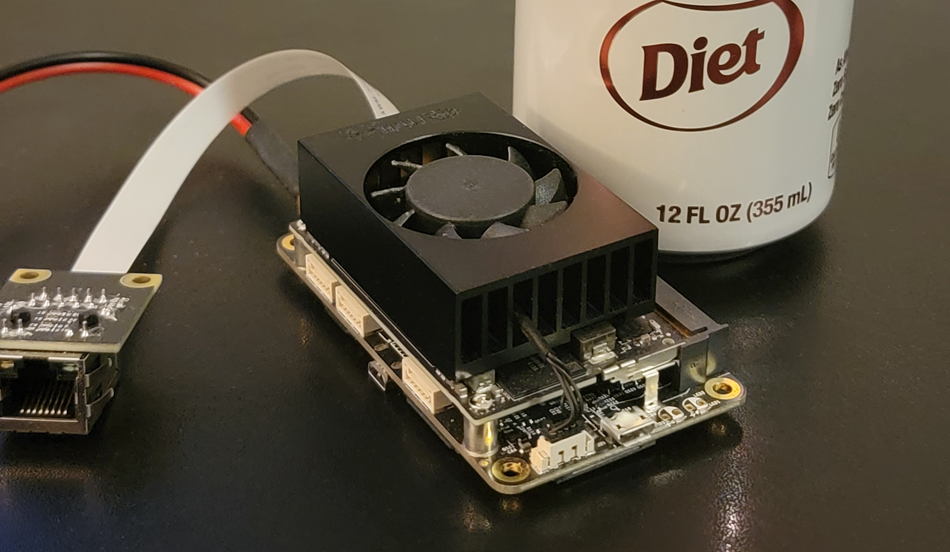
\includegraphics[width=1\linewidth]{orin-nx.png}
    \caption{The system under test. Every edge number in Section V was measured on this board — a Jetson Orin NX 16GB on its carrier board (fan attached), 355 mL can for scale. The compute module itself is 69.6 × 45 mm, smaller than a credit card; this is the entire machine that answers 0.65 s after end of speech.}
    \label{fig:orin-nx}
\end{figure}
Three processes, one GPU owner:

    \begin{itemize}
        \item voicecat + whisper.cpp (CUDA base.en): energy VAD, streaming transcription with LocalAgreement-2 commits, timestamp-based window trimming, barge-in (one byte stops the reply mid-stream). Committed words stream into the runner as typed text frames while the turn is still open.
        \item Gemma 4 on little-gemma: a $\sim$6,000-line C/CUDA runner for the Gemma 4 family (int8 tensor-core prefill, dp4a decode, GPU vision encoder, MTP speculative decoding, all quantizations byte-identical to the f32 reference by gate). The serve mode is a Unix-domain socket: connection = conversation, line = turn, typed frames ('T' text, 'I' image, 'A' audio) append to the open turn and prefill on arrival. A system-prompt file prefills once at server start (Section IV-C rides this).
        \item piper (VITS, en\_US voices) as a persistent stdin service on the CPU — the GPU belongs to the LLM. One ONNX call per line: first byte is roughly equal to whole-clause synthesis, 0.27–0.49 s per clause on the Orin's cores (18–26× realtime), 0.31 GB peak anonymous memory. Piper was chosen over Kokoro on speed (0.008 RTF vs $\sim$0.47-0.51 RTF) \cite{codesotatts}. CPU placement is measured, not assumed: on the A5000, CUDA piper loses to a desktop CPU at clause length (0.112 vs 0.089 s — the ONNX graph round-trips the bus 28 times for ops pinned to CPU, and launch/copy overhead swamps 20 MB of conv math) and only reaches 1.6× on long sentences; clause splitting (Section IV-C) moves TTS precisely into the regime where CPU wins, and on the Orin the iGPU would contend with decode for the same LPDDR5 anyway. Section IV-D removes the whole-clause wait itself: the same voice files, split at the latent boundary, stream first PCM in 0.10 s.
    \end{itemize}

Why external ASR when Gemma 4 is natively multimodal? Because we measured the native path and it fails three ways (see Section VII for details): the E2B/E4B conformer audio path confabulates rather than transcribes; the 12B hears speech but behaves as ASR-only for non-speech sound; and — the finding we could not have predicted — vision in context disables hearing on the 12B (seven arrangements tested, asymmetric, session-scoped, survives black frames). A voice+camera product on this family requires an external ASR lane; our pipeline's soundtrack policy (audio rides as a whisper transcript under the video span) is the direct product of that finding.

\section{Where the time goes, and how it is reclaimed}

\subsection{Metrics and protocol}


    \begin{itemize}
        \item TTFT: last user input → first reply token (server work becomes visible).
        \item TTFS / time-to-first-speakable: → first complete speakable unit (sentence, or clause once Section IV-C applies) — the unit the TTS can start on.
        \item TTFB (first audio): → first PCM sample out of the TTS. The number the ear judges. TTFT alone misorders systems: a fast first token followed by a 21-word sentence is slower to speak than a slower first token followed by a 6-word clause.
    \end{itemize}

All clocks are client-side (the runner is not trusted to grade itself), the first turn after model load is discarded (repack, clock ramp, draft-head warmup), and each measurement is a fresh conversation. Three delivery modes model the ASR: deferred (whole instruction arrives at turn end — the no-streaming baseline), burst (frames arrive as fast as the socket takes them), paced (30 words/s with 200 ms frame cadence — a real speaking rate). The 929-token spoken instruction (a long rambling preamble ending in a question) is the standard stimulus; replies must be byte-identical across delivery modes for a run to count (Section IV-B's lemma makes this achievable and it held in every reported cell, on both test machines).

\subsection{Prefill under speech}

Chunked prefill — a named scheduler feature in vLLM and TensorRT-LLM — splits a completed prompt so it can interleave with decode; llama.cpp's server has no such feature but likewise processes a prompt that has already arrived in full (ubatch splitting, prefix-cache reuse). In every serving stack we know, prefill begins only once the whole prompt is in hand. The open turn is different: while the user speaks, committed words are already immutable — LocalAgreement-2 commits exactly the prefix both hypotheses agree on — so their KV entries can be computed now, under the speech itself.

Correctness requires that tokenizing the turn in committed pieces equals tokenizing it whole. For SentencePiece this holds exactly when splits land on space boundaries: pieces never cross a space (the space glyph \_ starts pieces), so a word-boundary split cannot merge or reshape tokens across the seam. We verify, not just argue: equal token id sequences and byte-identical replies, deferred vs streamed, all three models. (One span of holdback is kept unprefilled to absorb ASR revisions of the most recent words; MSG\_PEEK lets the server prefill right up to the pending frame without consuming it.)

\begin{figure}[h]
    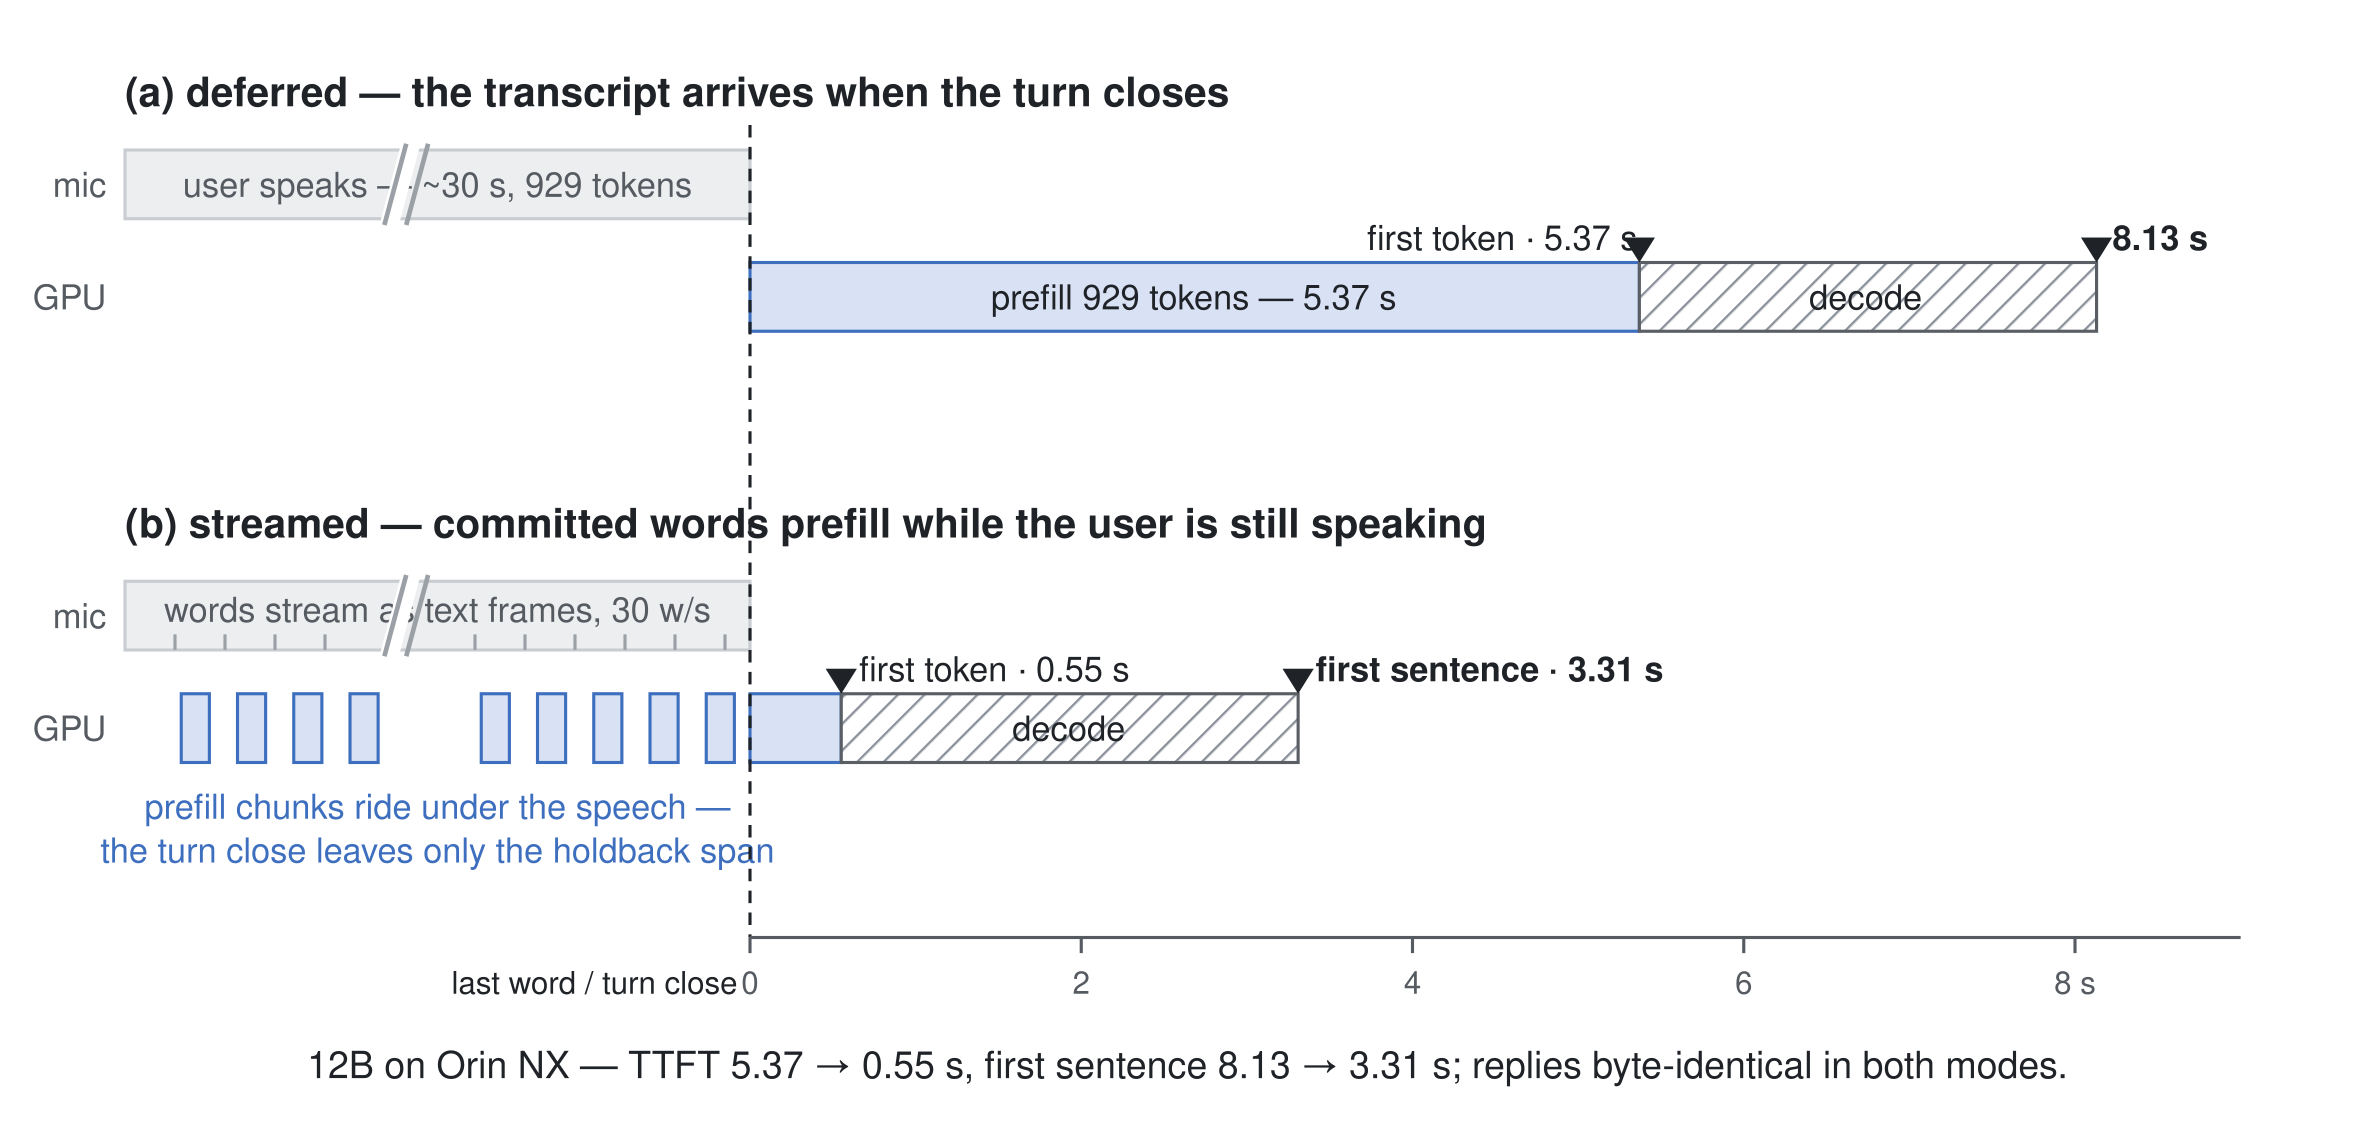
\includegraphics[width=1\linewidth]{fig-prefill-under-speech.png}
    \caption{In deferred delivery (a) the 5.37 s prefill starts only when the turn closes; streamed (b), committed words prefill during the speech itself and the turn close leaves only the holdback span — TTFT 5.37 → 0.55 s with byte-identical replies.}
    \label{fig:prefill-under-speech}
\end{figure}

\subsection{The LLM is the only clause splitter}

A streaming TTS layer flushes at punctuation. The baseline 2B, asked our standard question, answers in a single 21-word sentence with zero commas — there is nothing to flush until the sentence ends, 9.4 s of audio in one synthesis call. No glue-layer heuristic fixes this: splitting mid-clause produces unnatural speech, and only the model knows where a thought can pause. The split policy therefore lives in the model, installed as a system prompt loaded once at server start (prefilled once, zero per-turn cost):

\begin{quote}
    You are a voice assistant. Everything you write is spoken aloud by a text-to-speech engine, clause by clause, so write for the ear, not the eye. [...] Keep sentences short. Break long thoughts into clauses of five to ten words, separated by commas or periods [...] Get to the point in the first clause; details can follow.
\end{quote}

Effect on the E2B voice loop: first speakable unit 21 → 8 words (0.714 → 0.549 s), synthesis of that unit 0.49 → 0.27 s (VITS synthesis is $\sim$linear in audio length, so shorter first units pay twice), first audio 1.21 → 0.82 s. Two honest notes travel with this: style pressure sharpens a small model into confident error (the 8-word answer contains a wrong date; the vague baseline was defensible), and prompt-only is the bootstrap — the production path is a light finetune for human pause placement, which is often shorter than grammatical clauses.

\subsection{Streamer vocoder from stock voices}

After Section IV-B and IV-C, the TTS call itself is 30–50\% of what remains: VITS synthesizes a whole clause in one ONNX call, so first PCM waits for all of it. The fix exploits an asymmetry inside the model. The text encoder, duration predictor, and flow must see the whole clause — prosody is global — but they are cheap; the HiFi-GAN upsampler is most of the compute and is a pure convnet: finite receptive field, no attention, no recurrence. Anything with a finite receptive field can be decoded in overlapped chunks whose interiors are exact.

piper ships monolithic ONNX files, but the graph names its decoder, and exactly one tensor crosses into it (the masked latent feeding the decoder's input conv). Our splitter finds that boundary automatically and extracts encoder/decoder halves from any stock voice file — no retraining, no re-export; verified identical on an official voice and on our own finetune. At overlap R=16 frames the chunked decode saturates at max sample difference 4e-7 vs the monolithic output (fp32 noise), on both test machines. The streaming service (a drop-in for piper --output-raw) then emits 0.12 s chunks as they decode. The implementation ships in our piper fork as python -m piper.split plus a --stream CLI flag and synthesize\_stream() API, with an exactness test suite; it is a candidate for an upstream contribution.

End-to-end on the Orin, everything included (phonemization, encoder, first chunk, pipe): first PCM 0.10 s where the monolithic call took 0.27 s (voice-sys clause) — and 0.15 s even for a 21-word sentence whose monolithic call took 0.49 s. First byte is now O(1) in clause length; synthesis continues at 6–13× realtime under playback. The techniques compose: first audio 1.21 → 0.82 (Section IV-C) → 0.65 s. One trade is inherent: streamed chunks cannot be peak-normalized (that needs the whole clause), so the service ships the voice's native level. This is the one architectural idea the cascade borrows from speech-native models: their codecs stream by construction; ours now does too.

\subsection{Speculative decoding as a latency and battery feature}
Gemma 4's first-party MTP head drafts the next N tokens; greedy verification makes output byte-identical to plain decoding by construction — only tokens/s and acceptance move. What it is worth is sharply content-dependent (block-3, serve mode, steady-state): structured output $\sim$2× (12B A5000 2.16×, Orin 1.85×, 100\% acceptance), free prose 1.10–1.35× (the 12B's 1024-wide head lands $\sim$49\% of prose drafts; E4B's 256-wide head $\sim$30\%). We report the distribution, not a flat multiplier — flat claims in the spec-decoding literature do not survive contact with prose. On the battery angle: MTP cuts energy per token from 2.85 to 2.29 J/token on the Orin (the GPU is bandwidth-bound; fewer full passes per token is less DRAM traffic) — for a robot, spec decoding is a battery feature before it is a latency feature.

\subsection{The substrate, briefly}
None of Section IV-B–IV-E works if the kernels are slow. The runner's prefill is an int8 tensor-core (mma) path with warp-cooperative activation quantization and flash-attention prefill; decode is dp4a with split-K attention, frozen kernels, and CUDA-graph capture; weights are zero-copy on the integrated GPU (host and device share LPDDR5 — copying would hold every byte twice), mmap'd and unpinned where the quantization is repacked anyway. Every optimization is gated byte-identical against a f32 reference and, for the speculative path, by acceptance-rate tripwires (which caught three real bugs). Full engineering logs, including the falsified dead ends, are in the repository journals \cite{littlegemma}. The result on the Orin: $\sim$0.8× of llama.cpp's prefill throughput and 1.17–1.26× its decode, from a codebase a single reviewer can actually read ($\sim$6,000 lines).

\section{Evaluation}

\subsection{Setup}
Orin NX 16GB, JetPack 6.2.1, pinned clocks for benchmarks (jetson\_clocks; production ships DVFS — a reboot resets the pin, and every number here was re-verified against that trap), models: Gemma 4 12B-it Q4\_K\_M, E4B-it Q4\_K\_M, E2B-it QAT q4\_0 (Google's quantization-aware release), each with its MTP head; whisper.cpp CUDA base.en; piper en\_US voices. Cross-silicon: RTX A5000 (Windows) + i7-8086K. All measurements are client-side per Section IV-A.

\subsection{The substrate vs llama.cpp}

\begin{table}[H]
    \begin{tabularx}{\columnwidth}{l X X X}
        device & model  & little-gemma  & llama.cpp \\
        Orin & 12B & 173 & 0.80×\\
        Orin & E4B & 417 & 0.82×\\
        Orin & E2B QAT & 815 & 0.80×\\
    \end{tabularx}
    \caption{Serve-mode prefill, tok/s (929-token turn, warm)}
    \label{tab:serve-mode-prefill}
\end{table}


\begin{table}[H]
    \begin{tabularx}{\columnwidth}{l X X X X}
        device & model  & little-gemma  & llama.cpp & ratio\\
         Orin & E4B & 16.80 & 13.36 & 1.26×\\
         Orin & 12B & 8.27 & 7.04 & 1.17×\\
    \end{tabularx}
    \caption{Plain decode, tok/s (256 tokens, warm; llama-bench reference)}
    \label{tab:plain-decode}
\end{table}

MTP multiplies on top (Section IV-5). Where the design point shows is multimodal turns: little-gemma reaches first-sentence on an image+question turn in 1.98 s (E4B) / 5.22 s (12B) on the Orin vs 35.8 / 98.6 s for llama-server (which burns its lead in an unsuppressed thinking channel and host-side encode) — the raw-token-stream server and encode-off-critical-path choices are TTFB choices, not throughput choices.

\subsection{The dictation matrix (Orin)}


\begin{table}[H]
    \begin{tabular}{ccc}
        model & deferred & paced (30 w/s) \\
        12B & 5.37 / 8.13 & 0.55 / 3.31 \\
        E4B & 2.23 / 3.20 & 0.26 / 1.24 \\
        E2B QAT & 1.15 / 1.76 & 0.10 / 0.72\\
    \end{tabular}
    \caption{929-token spoken instruction; TTFT / TTFS in seconds}
    \label{tab:929-token}
\end{table}

(Burst delivery pays frame padding and is dominated by deferred — measured, not assumed; deferred runs reproduce to the millisecond.)

\subsection{End-to-end: the 0.65 s anatomy}

\begin{figure}[H]
    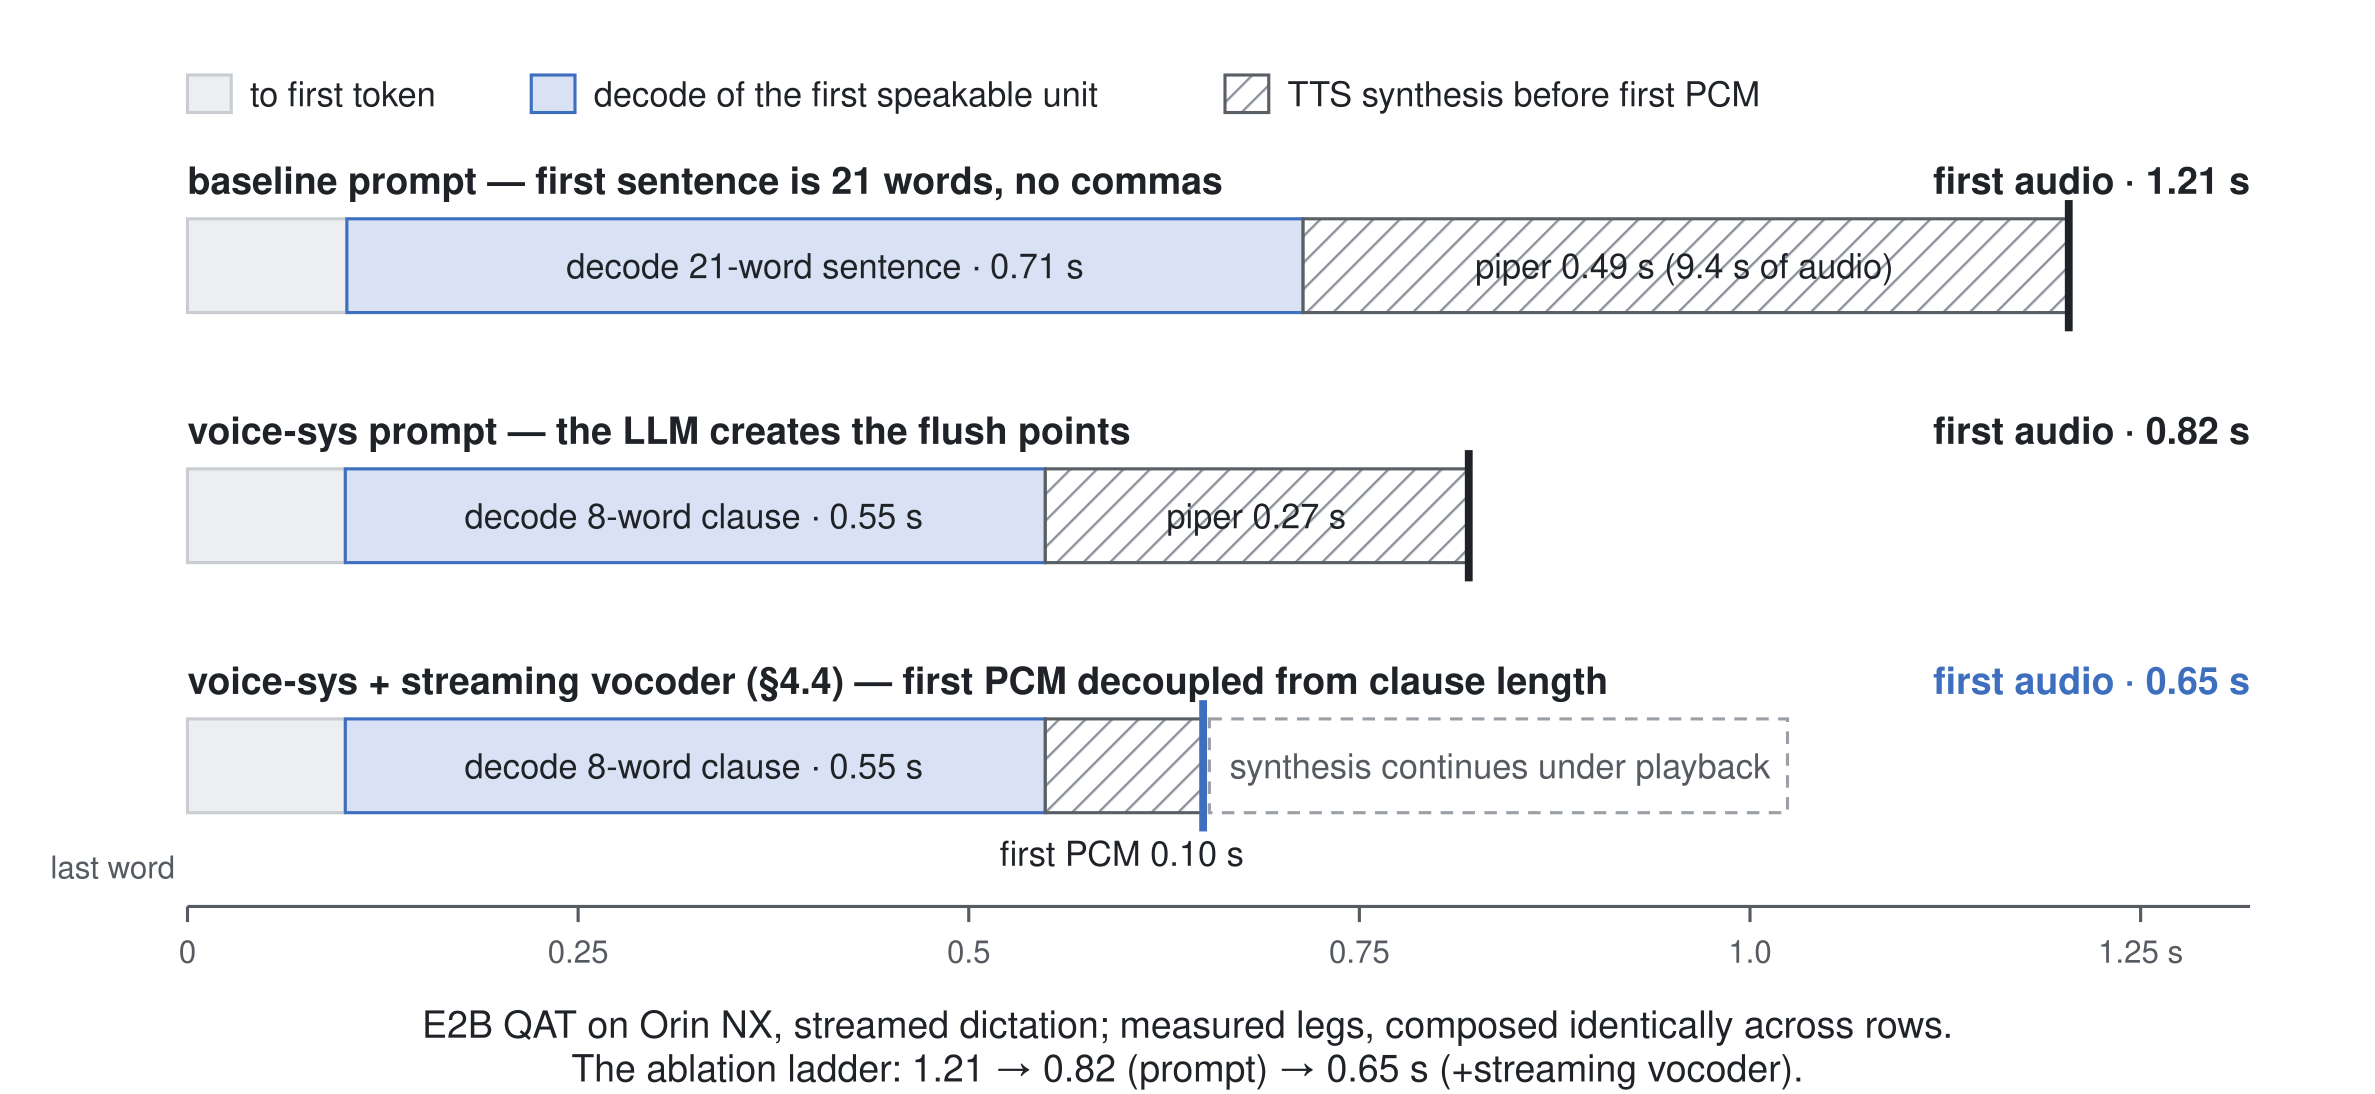
\includegraphics[width=1\linewidth]{fig-first-audio-anatomy.png}
    \caption{The same question, three configurations. The voice-sys prompt cuts the first speakable unit from 21 to 8 words (1.21 → 0.82 s); the streaming vocoder (Section IV-D) then decouples first PCM from clause length entirely (0.82 → 0.65 s). Synthesis continues under playback.}
    \label{fig:first-audio-anatomy}
\end{figure}

With whisper.cpp's final-commit pass in the loop (base.en CUDA, $\sim$0.55 s per invocation, invocation-cost-dominated), voicecat closes the turn $\sim$1.0 s after end of speech in live-mic operation; a persistent whisper server, amortizing that load-dominated invocation cost across passes, is the identified upgrade path. We expect it to pull live-mic TTFB toward the streamed-dictation number but have not measured it (Section VIII).

\begin{table}[H]
\centering
\small
\begin{tabularx}{\columnwidth}{l X X X}
\hline
Tier & Intelligence & TTFB & Experience \\
\hline
12B &
Strongest open-weight $\leq$16\,GB &
3.4\,s &
Common experience (P90). \\

E4B &
High &
1.35\,s &
Below the industry median (1.4--1.7\,s). \\

E2B QAT &
Good &
0.65\,s &
Within the theoretical ideal; rarely achieved in production. \\
\hline
\end{tabularx}
\caption{Three conversational operating points on a single Jetson Orin NX. TTFB is approximated as TTFS + TTS latency.}
\label{tab:three-tiers-exp}
\end{table}

\begin{figure}[H]
    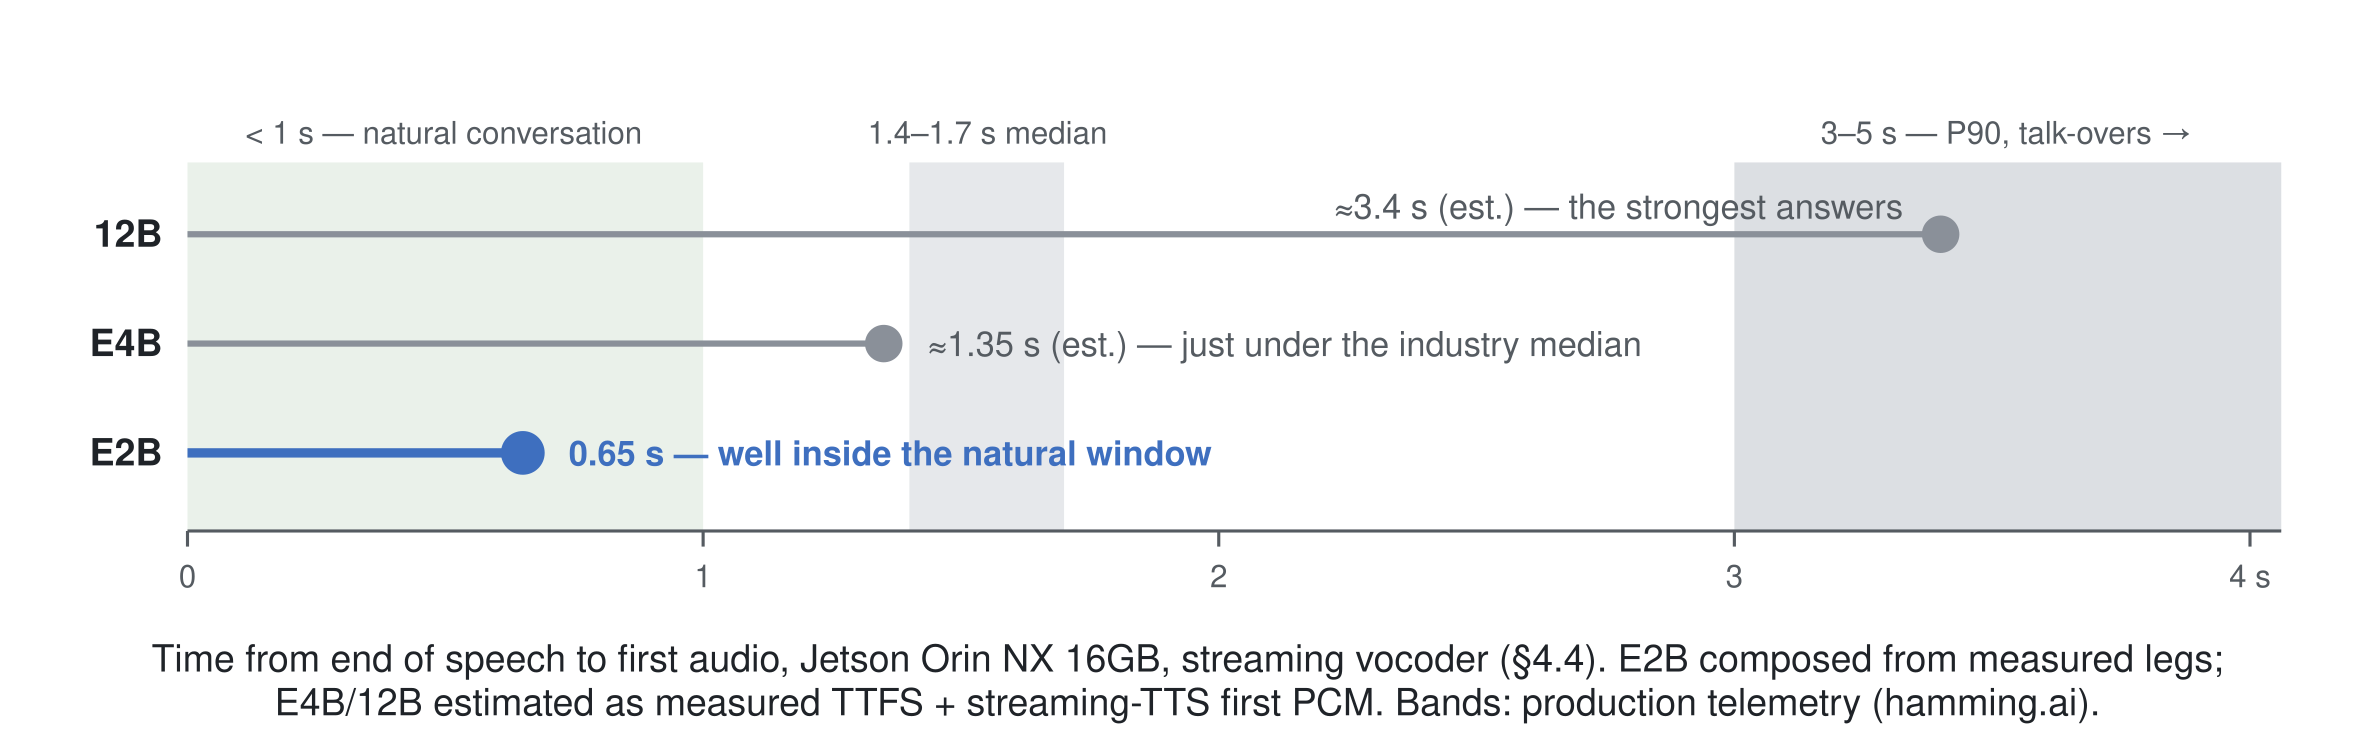
\includegraphics[width=1\linewidth]{fig-tiers-vs-industry.png}
    \caption{One board, one pipeline, three operating points. The E2B tier lands inside the natural-conversation window that production telemetry reports as rarely achieved; the E4B matches the industry median; the 12B trades latency for the strongest answers.}
    \label{fig:tiers-vs-industry}
\end{figure}

The tier table is the product story: the same hardware and pipeline lets a robot answer trivia with the 12B and do fluent small talk with the E2B — switching is a model file, not an architecture.

\subsection{Memory: does it fit an 8 GB Nano?}
Measured the honest way for Jetson (anonymous RSS + nvmap; VmHWM counts evictable file pages and MemAvailable under-counts nvmap — both mislead): little-gemma E2B QAT serve 3.2 GB unreclaimable (nvmap 3.00 + anon 0.11, after mmap'ing the weight blob and skipping the pin for fully-repacked models: 5.5 → 3.2 GB), whisper $\sim$0.7 GB, piper 0.31 GB peak → $\approx$ 4.2 GB for the full voice stack, leaving $\sim$2.2 GB slack on a 7.4 GB-usable headless Nano, with room for the vision encoder ($\sim$0.7 GB). Caveat, stated plainly: measured on the NX 16GB against an 8 GB budget, not yet on the Nano SKU.

\subsection{Power}
GPU-saturated decode peaks $\sim$23 W (default profile; 40 W MAXN raises clocks but the workload is bandwidth-bound), idle-to-peak on a supply a robot already carries. MTP reduces J/token 2.85 → 2.29 (Section IV-E). Moshi's reference deployment is an L4 (24 GB, $\sim$72 W TDP) datacenter GPU

\subsection{Cross-silicon: the cascade vs Moshi on Moshi's hardware class}
\begin{table}[H]
    \centering
    \small
    \begin{tabular}{ccccc}
       model  &  1st token & 1st clause & +piper & word → audio \\
        12B &  0.090& 0.241 & 0.109&0.35 s\\
        E4B & 0.065 & 0.132 & 0.108&0.24 s\\
        E2B QAT & 0.121& 0.29 & 0.193 	&0.48 s\\
    \end{tabular}
    \caption{Moshi on our A5000: $\sim$0.13 s TTFB warm. Our pipeline on the same card (+ i7-8086K for piper), same protocol as Section V-C}
    \label{tab:pipeline}
\end{table}

Three readings. (1) The remaining 2–4× is structural: a speech-native model starts vocoding without waiting for a speakable text unit; the cascade's floor is one decoded clause plus one VITS call ($\sim$0.2 s). (2) Model size has almost stopped mattering — 2B to 12B spans first-clause 0.13–0.29 s once streaming hides prefill; content dominates (the E2B is slowest end-to-end because its clause contains a date that verbalizes to 3.9 s of audio). (3) The datacenter card + desktop CPU beat the 20 W board by only $\sim$1.7× end-to-end (0.48 vs 0.82 s, monolithic-TTS configurations — the streaming vocoder shipped after this study and tightens both sides): the conversational regime is floor-bound, not compute-bound, which is precisely the regime where an edge deployment loses nothing that matters.

\subsection{Same board, same brain: the cascade baseline}
The cleanest ablation of our techniques is another cascade with everything else held equal. HuggingFace's speech-to-speech pipeline ran on the same Orin NX against the same Gemma E2B QAT weights (served by an unmodified llama-server on the GPU; faster-whisper and MMS-TTS on CPU — the same ears/mouth placement we chose, reached there by necessity since PyPI CUDA wheels cannot see the Tegra iGPU). End of speech → first reply audio, live-paced 16 kHz socket input, warm medians:


\begin{table}[H]
\centering
\begin{tabular}{>{\raggedright\arraybackslash}p{2cm}cc}
\hline
pipeline & warm TTFB & spread \\
\hline
HF speech-to-speech, defaults & 1.6 s & 0.7--1.7 s \\
HF speech-to-speech, tuned (sentence batch 1) & 0.9 s & 0.7--1.7 s \\
ours (Section V-D) & 0.65 s & reproducible legs \\
\hline
\end{tabular}
\end{table}

The remaining difference is precisely the paper's contribution list run in reverse: their chain is serial after end of speech — a full ASR pass, a full prompt prefill, the first sentence's decode, and a whole-first-sentence VITS synthesis (their default even batches THREE sentences before the first TTS call; changing that one number is the 1.6 → 0.9 difference). Their first-audio latency therefore scales with reply length, where ours is $\sim$O(1) after Section IV-B–IV-D. VAD hang time is not the story on either side (their silence threshold is 64 ms).

Two qualifications, both in their favor and against. Their flagship TTS backends (Qwen3-TTS via CUDA-graph codec decoding, Kyutai's Pocket) do stream natively — the whole-sentence behavior we measured is their CPU-viable tier — but the streaming tier is a different model architecture wanting a GPU, not a retrofit onto stock voices like Section IV-D. And their measured 0.9 s carried an artificially light ASR leg: the VAD only captured $\sim$0.9 s fragments of our synthetic-voice question. On long input the comparison collapses entirely: a 31.8 s natural spoken question is segmented at breath pauses and answered INTO the user's ongoing speech (first audio 25–28 s before end of speech), and even with perfect segmentation the post-speech chain scales with utterance length (their ASR leg alone measures 3.9 s for 31.8 s of audio on this CPU) — where prefill-under-speech holds ours at 0.65 s regardless (Section IV-B's 929-token case is the measured proof).

Figure 5 makes the divergence explicit. We swept six spoken questions of increasing length (3.8–32 s, synthesized and measured on the same board) and clocked each leg. Our prefill term is flat — and, at these lengths, nearly free in either placement: streamed ttft stays at 0.09–0.12 s across the range, and even a deferred one-shot prefill of the 90-word question costs 0.20 s. Natural speech arrives at $\sim$3 tokens/s against a prefill rate of $\sim$800 (E2B); anything a user can say in a turn is cheap to prefill. What the open turn hides at conversational lengths is therefore the ASR pass, not the prefill — prefill hiding earns its keep at dictation lengths and on the slower 12B tier (Section IV-B). The HuggingFace floor is not a line we could measure end-to-end — its VAD replies into our synthetic speech past $\sim$15 s — so we compose its best case: the measured faster-whisper base-int8 ASR pass (1.20 s at 3.8 s of audio, rising to 3.52 s at 32 s) plus a 0.45 s downstream constant (prefill, first-sentence decode, first MMS-TTS call) anchored to their measured 0.9 s tuned point. Even granting perfect segmentation, the floor rises from $\sim$1.6 s at a 5 s prompt to $\sim$3.9 s at 30 s. The gap the reader sees is the ASR placement: run serially after end of speech it scales with the utterance; committed during speech it costs one final pass, a constant. Everything else — the LLM prefill, the first speakable unit's decode, the vocoder — is constant in prompt length on both sides; the size of those constants (clause-first flushing, the streaming vocoder) is Section IV-C–IV-D's fight, already settled in Figure 3.

\begin{figure}[H]
    \centering
    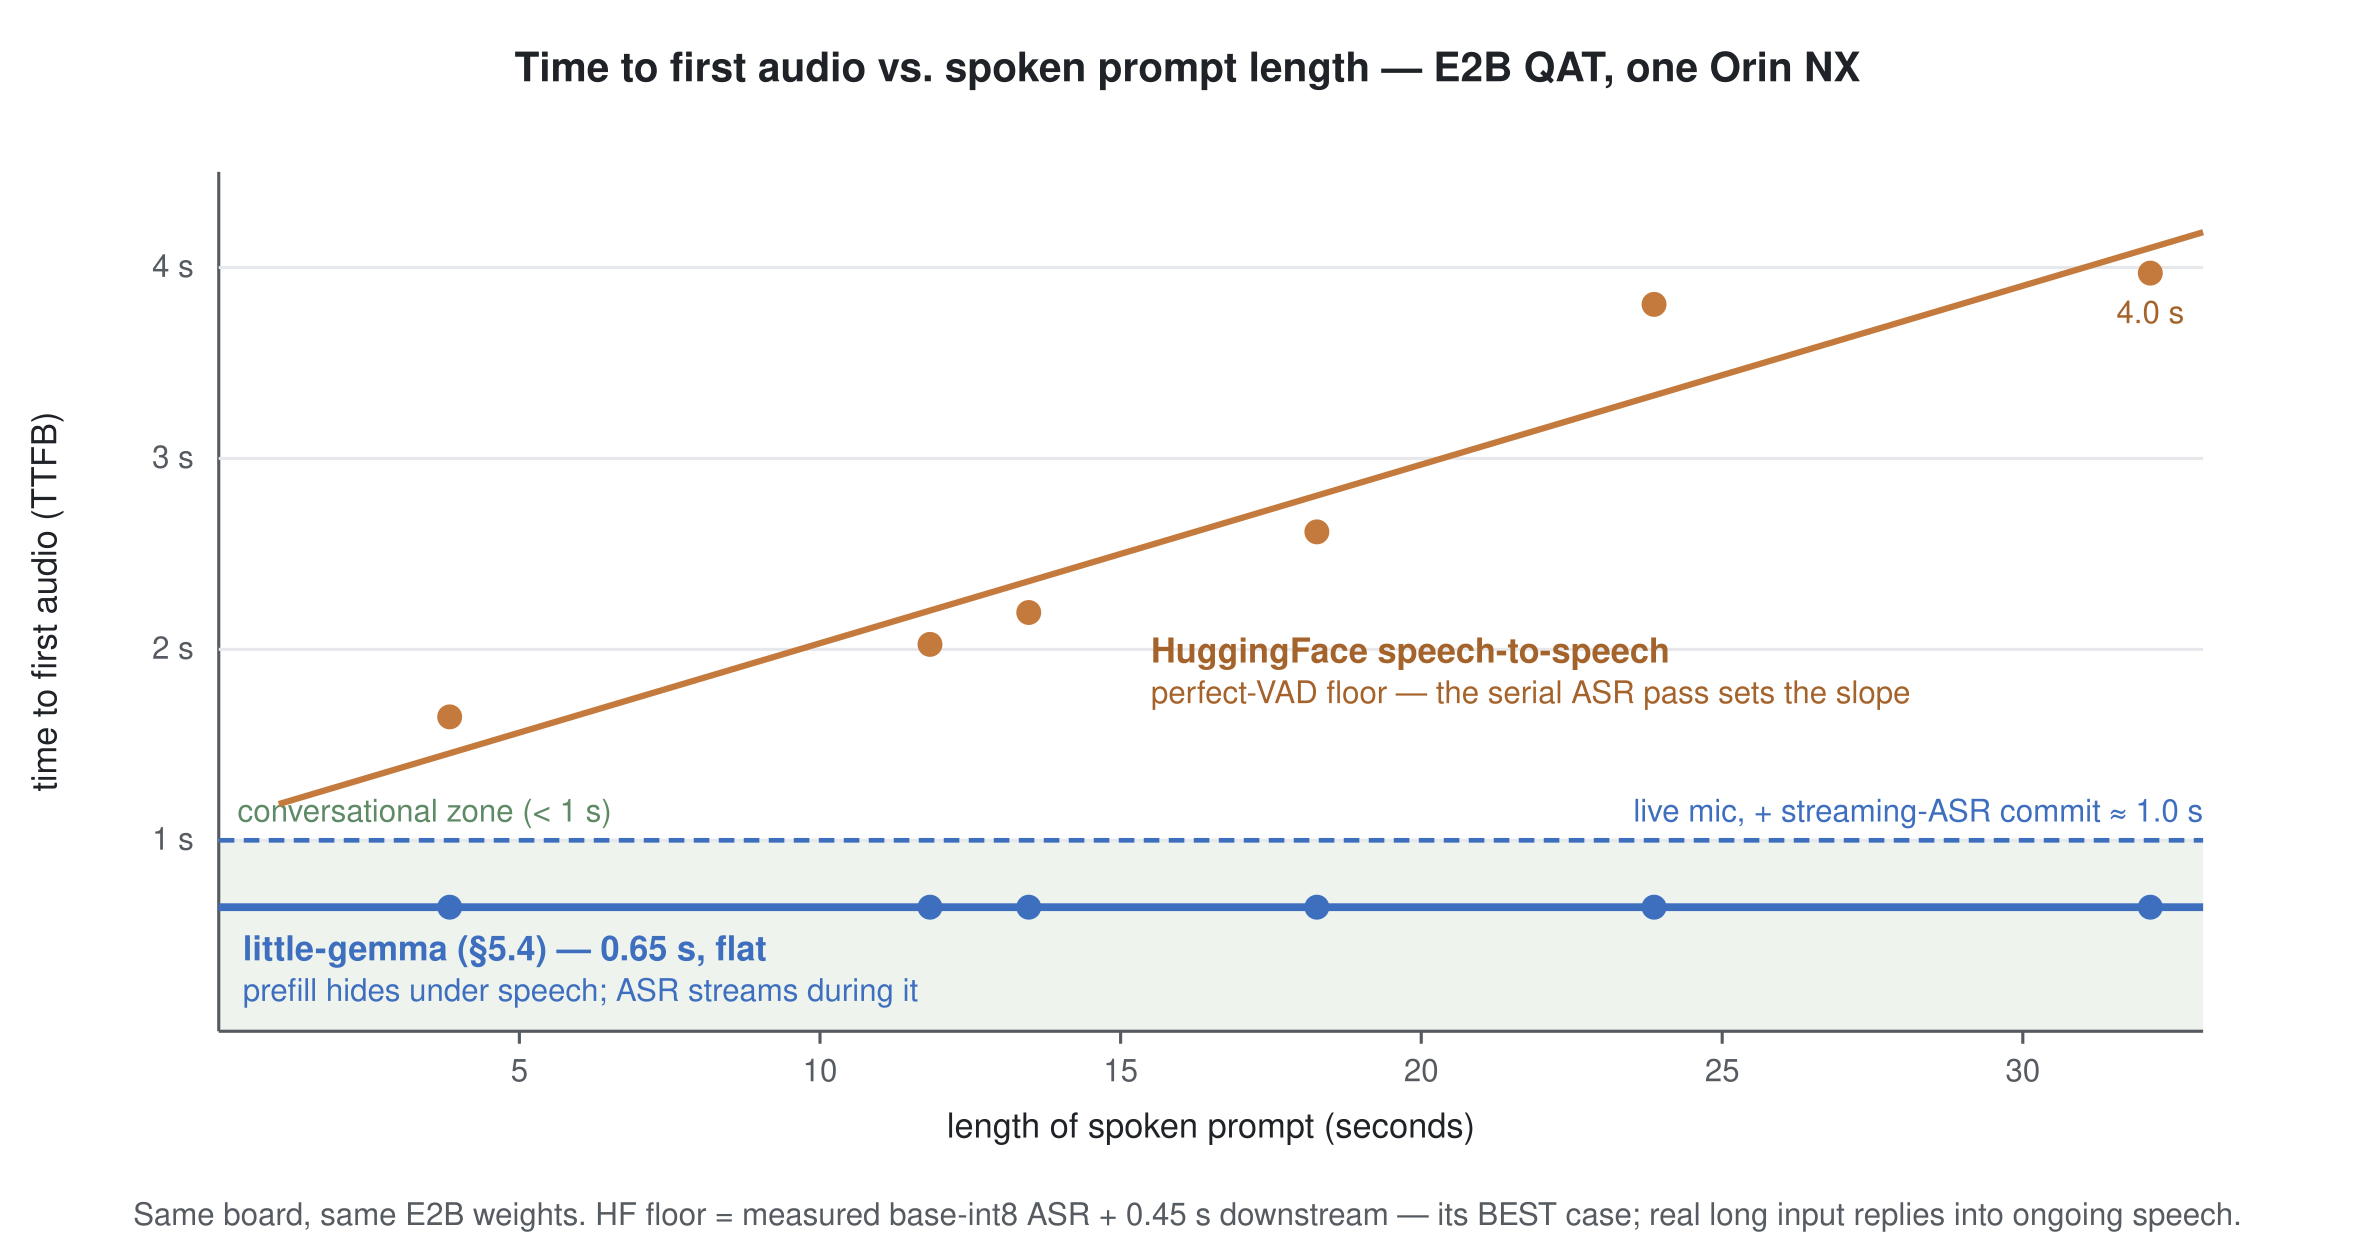
\includegraphics[width=1\linewidth]{fig-ttfb-vs-length.png}
    \caption{The same board and E2B weights, swept over prompt length. Our TTFB is flat (0.65 s streamed-text; $\approx$1.0 s live-mic once the streaming-ASR final commit is included, still inside the conversational band). The HuggingFace perfect-VAD floor rises with the serial ASR pass. Points are measured; the HF line is its best case — real long input replies into ongoing speech, which is worse than the floor shown.}
    \label{fig:ttfb-vs-length}
\end{figure}

\subsection{Session aging: does it hold as the context fills?}
A fair question the single-turn numbers do not answer: does responsiveness decay over a long conversation as the 8K window fills? We measured it directly — one persistent E2B QAT session on the Orin (plain serve, no MTP, pinned clocks, SoC otherwise idle), driven turn after turn with fixed $\sim$178-token turns until the server reported the context full, which happened after 42 turns ($\sim$7,475 tokens).
\begin{figure}[H]
    \centering
    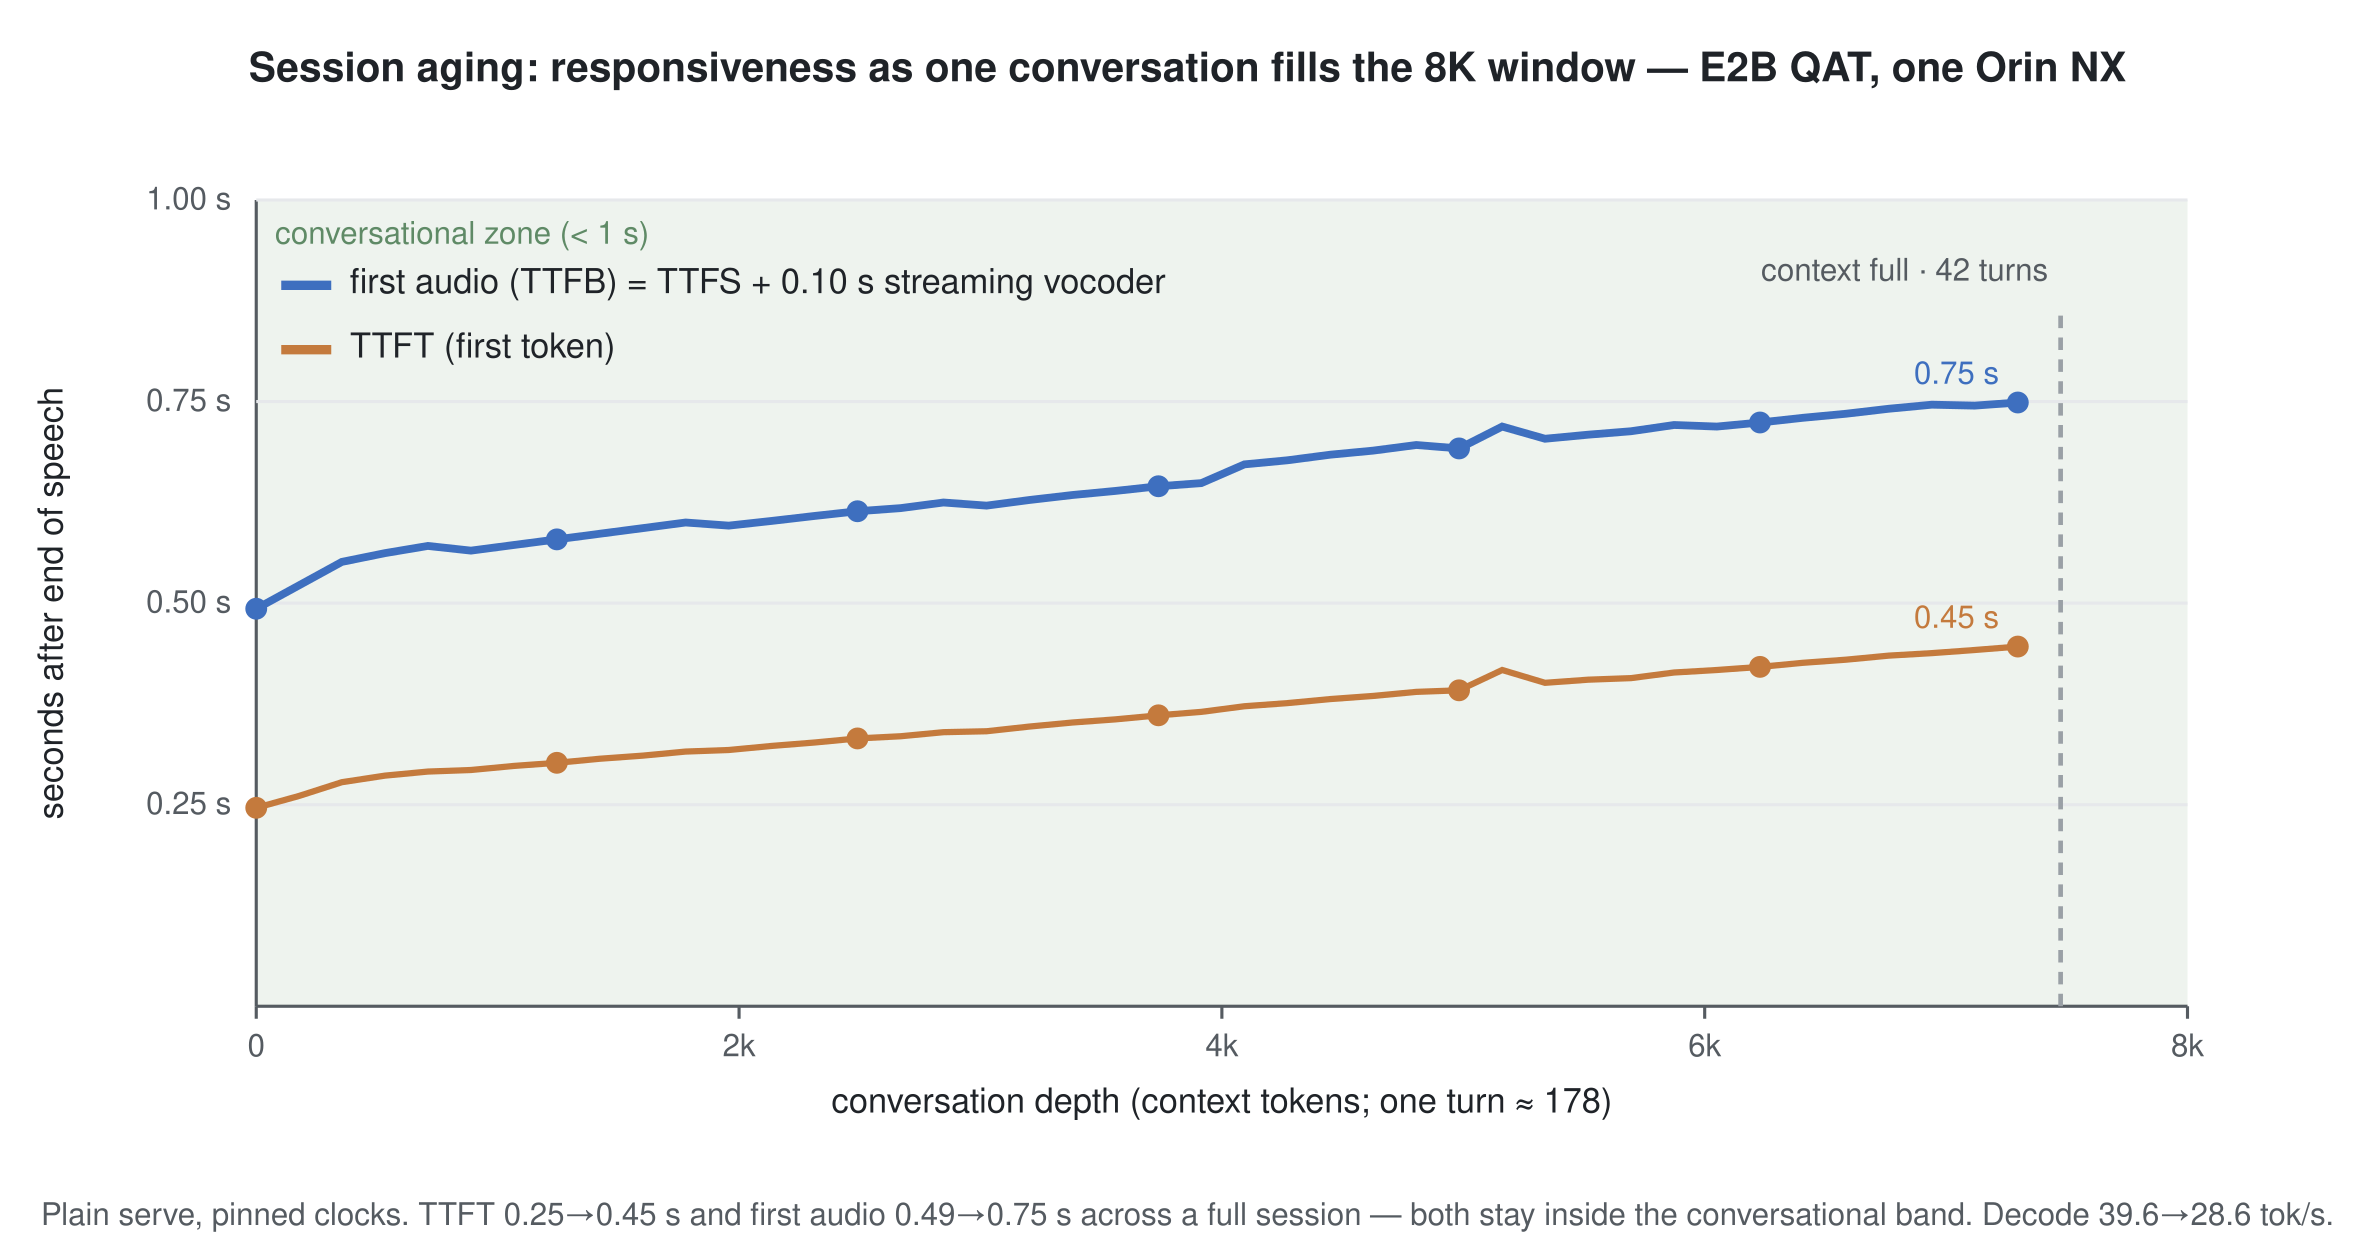
\includegraphics[width=1\linewidth]{fig-session-aging.png}
    \caption{TTFT and first audio (measured TTFS + the streaming vocoder's 0.10 s first-PCM constant, Section IV-D) as one conversation fills the window. Both rise gently and slightly sub-linearly — TTFT 0.25 → 0.45 s, first audio 0.49 → 0.75 s — and both stay inside the conversational band for the entire session. Plain decode slows 39.6 → 28.6 tok/s (attention over the growing KV), still far above the $\sim$3 tok/s real-time-listening floor (Section VI).}
    \label{fig:session-aging}
\end{figure}

The growth is bounded because most layers use sliding-window attention — their cost is window-bounded and constant — so only the global layers pay for the accumulating KV. Absolute values reflect this fixed short-turn stimulus, chosen to fill the context at a constant rate; the load-bearing result is the slope: a full session adds only $\sim$0.2 s to TTFT and $\sim$0.26 s to first audio, and the pipeline still answers in under 0.75 s at context-full. The design point holds across the whole session, not just the first turn.

\section{Discussion}
What the cascade buys for its $\sim$0.5 s of structural disadvantage: the brain is a commodity part. The same pipeline ran three Gemma 4 variants (E2B, E4B, 12B) without retraining anything; it processes a camera feed with the same open-turn mechanics that stream dictation (Section IV-B); it speaks Gemma's full tool-calling protocol because the server passes control tokens through; and its answer quality is that of a 12B instruction-tuned text model, not what survived speech-topology training. Fluency, meanwhile, turned out not to require a new species of model — just refusing to waste the time the user's own speech provides, and letting the model place its own pauses.

The A5000 study reframes the edge question. The usual framing is "how much worse is edge?"; measured, the answer in this regime is 1.7× on latency, at 1/6th the power class — because the floor is set by clause decoding and vocoding, not by FLOPs. TTFB pursuit and throughput pursuit diverge here: past the point where prefill hides under speech and decode outruns speech playback ($\sim$3 tok/s suffices for real-time listening; even the 12B's 8.3 tok/s clears it), more tokens/s stops buying experienced fluency. That is why this work no longer competes with llama.cpp on llama.cpp's axis — and why a 6,000-line runner can hold the design point at all.

\section{Limitations}

    \begin{itemize}
        \item The dictation TTFB excludes the ASR final-commit pass (Section V-D gives the live-mic number, $\sim$1.0 s to turn close); Moshi's number includes its hearing. The persistent-whisper upgrade path narrows this and is measured future work.
        \item The Moshi comparison is anchor-mismatched in Moshi's favor and ours at once: its probe clock starts at the start of input streaming (fed silence, the full-duplex model initiates speech itself), ours at the end of user speech. Full-duplex design bounds Moshi's turn response by roughly the same loop latency, so the citation is fair in spirit, but the rigorous head-to-head — stream a recorded question, anchor at its final word — remains future work. (The handshake question is resolved: excluded by construction.)
        \item Style pressure makes the 2B confidently wrong where it was vaguely right (Section IV-C); the clause-splitting prompt trades a quality edge for fluency at the smallest tier. Finetuning may recover both.
        \item All benchmarks use greedy decoding (the byte-identity discipline requires it). Sampling exists and composes with MTP distribution-exactly — the verify samples the target's distribution and accepts a draft only on agreement, so speculation never alters the output distribution — but acceptance drops (76.6\% → 28–46\% at temperature 1.0 on the 2B) and sampled-mode latency/quality is not separately characterized here.
        \item Single-user, single-stream serving; no batching story.
        \item 8 GB verdict extrapolated from the NX 16GB (Section V-F).
        \item Gemma 4's native audio path is not usable as the pipeline's ears, which is what makes the whisper lane load-bearing rather than a fallback. The capability boundary we measured (greedy decoding; Orin + A5000):
    \end{itemize}

    \begin{table}[H]
    \small
    \begin{tabularx}{\columnwidth}{lXX}
    \hline
    Configuration & Native-audio result & Status \\
    \hline
    E2B/E4B, speech &
    Confabulates; follows the \emph{prompt} rather than the audio. Coarse comprehension survives but verbatim ASR fails. &
    Model limitation; reproduced in the fork's tools and upstream \texttt{llama.cpp}. \\
    
    12B, speech only &
    Accurate ASR (JFK transcribed verbatim). &
    Usable for speech only. \\
    
    12B, non-speech only &
    Confabulates or denies; describes the instrument named in the prompt. &
    Music/ambient require an external tagger. \\
    
    12B + vision &
    Hearing disabled for all tested orderings; vision remains functional. &
    Use Whisper whenever vision is enabled. \\
    \end{tabularx}
    \caption{Native audio evaluation results.}
    \end{table}


\section{Future Work}

Finetune for human pause placement (shorter than grammatical clauses); persistent whisper service (flips the streaming-vs-endpass verdict unconditionally); integrate the streaming vocoder (Section IV-D) into the live-mic loop and re-measure the composed 0.65 s as one system; re-run the A5000 cross-silicon table with streaming TTS on both sides; Nano 8GB SKU validation; barge-in latency characterization; camera+voice concurrent sessions (the A/V exclusion policy exists, the latency study does not).

\section{Conclusion}

Fluent and cohesive do not require choosing. A 20 W board running unmodified open-weight models answers 0.65 s after you stop talking — because the pipeline stops wasting the seconds the user's own speech offers (prefill under speech), lets the model create the places speech can begin (the LLM as clause splitter), and measures the thing the ear actually judges (TTFB, not TTFT). The gap to purpose-trained speech-to-speech models is real, structural, and — at 2–4× against a species that cannot swap its brain, read a camera, or call a tool — a good trade for most embodied products.


% if have a single appendix:
%\appendix[Proof of the Zonklar Equations]
% or
%\appendix  % for no appendix heading
% do not use \section anymore after \appendix, only \section*
% is possibly needed

% use appendices with more than one appendix
% then use \section to start each appendix
% you must declare a \section before using any
% \subsection or using \label (\appendices by itself
% starts a section numbered zero.)
%


\appendices
\section{Reproducibility}
Every number traces to a committed harness: the repository's \verb|bench/| directory carries the dictation clients (client-side clocks, three delivery modes), the standard 929-token stimulus, the TTS timing scripts, the memory samplers (anon+nvmap), the serve-prefill bench harnesses for both machines, and the clause-flushing glue that makes the pipeline a single shell command; docs/voice-pipeline.md is the runnable reproduction guide (exact command lines, protocol rules, and the honest gaps). The streaming vocoder ships in our piper fork (split tool + streaming API + tests). The engineering journals include the falsified attempts. Replies are byte-identical across delivery modes and quantization levels by gate.


% Can use something like this to put references on a page
% by themselves when using endfloat and the captionsoff option.
\ifCLASSOPTIONcaptionsoff
  \newpage
\fi



% trigger a \newpage just before the given reference
% number - used to balance the columns on the last page
% adjust value as needed - may need to be readjusted if
% the document is modified later
%\IEEEtriggeratref{8}
% The "triggered" command can be changed if desired:
%\IEEEtriggercmd{\enlargethispage{-5in}}

% references section

% can use a bibliography generated by BibTeX as a .bbl file
% BibTeX documentation can be easily obtained at:
% http://mirror.ctan.org/biblio/bibtex/contrib/doc/
% The IEEEtran BibTeX style support page is at:
% http://www.michaelshell.org/tex/ieeetran/bibtex/
%\bibliographystyle{IEEEtran}
% argument is your BibTeX string definitions and bibliography database(s)
%\bibliography{IEEEabrv,../bib/paper}
%
% <OR> manually copy in the resultant .bbl file
% set second argument of \begin to the number of references
% (used to reserve space for the reference number labels box)
\begin{thebibliography}{18}

\bibitem{sharma2026latency}
S.~Sharma, ``Voice AI Latency: What's Fast, What's Slow, and How to Fix It,'' Hamming AI, Jan.~12, 2026. [Online]. Available: \url{https://hamming.ai/resources/voice-ai-latency-whats-fast-whats-slow-how-to-fix-it}. Archived at: \url{https://web.archive.org/web/20260511153827/https://hamming.ai/resources/voice-ai-latency-whats-fast-whats-slow-how-to-fix-it}

\bibitem{hamming2026metrics}
Hamming AI, ``Voice Agent Evaluation Metrics: Definitions, Formulas \& Benchmarks,'' Jan.~18, 2026. [Online]. Available: \url{https://hamming.ai/resources/voice-agent-evaluation-metrics-guide}. Archived at: \url{https://web.archive.org/web/20260707200723/https://hamming.ai/resources/voice-agent-evaluation-metrics-guide}

\bibitem{defossez2024moshi}
A.~Défossez, L.~Mazaré, M.~Orsini, A.~Royer, P.~Pérez, H.~Jégou, E.~Grave, N.~Zeghidour, ``Moshi: A speech-text foundation model for real-time dialogue,'' \emph{arXiv preprint arXiv:2410.00037}, 2024. [Online]. Available: \url{https://arxiv.org/abs/2410.00037}

\bibitem{stivers2009turntaking}
T.~Stivers, N.~J.~Enfield, P.~Brown, C.~Englert, M.~Hayashi, T.~Heinemann, G.~Hoymann, F.~Rossano, J.~P.~de~Ruiter, K.-E.~Yoon, and S.~C.~Levinson, ``Universals and cultural variation in turn-taking in conversation,'' \emph{Proceedings of the National Academy of Sciences}, vol.~106, no.~26, pp.~10587--10592, 2009. doi:10.1073/pnas.0903616106.

\bibitem{kyutai2024moshirepo}
Kyutai Labs, ``Moshi,'' GitHub repository. [Online]. Available: \url{https://github.com/kyutai-labs/moshi}

\bibitem{nvidial4}
NVIDIA, ``NVIDIA L4 Tensor Core GPU,'' Datasheet. [Online]. Available: \url{https://www.nvidia.com/en-us/data-center/l4/}

\bibitem{xie2024miniomni}
Z.~Xie and C.~Wu, ``Mini-Omni: Language models can hear, talk while thinking in streaming,'' \emph{arXiv preprint arXiv:2408.16725}, 2024. [Online]. Available: \url{https://arxiv.org/abs/2408.16725}

\bibitem{xie2024miniomni2}
Z.~Xie and C.~Wu, ``Mini-Omni2: Towards open-source GPT-4o with vision, speech and duplex capabilities,'' \emph{arXiv preprint arXiv:2410.11190}, 2024. [Online]. Available: \url{https://arxiv.org/abs/2410.11190}

\bibitem{pipecat}
Pipecat (Daily), GitHub repository. [Online]. Available: \url{https://github.com/pipecat-ai/pipecat}

\bibitem{livekitagents}
LiveKit, ``Agents,'' GitHub repository. [Online]. Available: \url{https://github.com/livekit/agents}

\bibitem{hfspeech2speech}
Hugging Face, ``speech-to-speech (v0.2.10),'' GitHub repository. [Online]. Available: \url{https://github.com/huggingface/speech-to-speech}

\bibitem{llamacpp}
G.~Gerganov \emph{et al.}, ``llama.cpp: LLM inference in C/C++,'' GitHub repository. [Online]. Available: \url{https://github.com/ggml-org/llama.cpp}

\bibitem{machacek2023whisper}
D.~Macháček, R.~Dabre, and O.~Bojar, ``Turning Whisper into real-time transcription system,'' \emph{arXiv preprint arXiv:2307.14743}, 2023. Presented at IJCNLP-AACL 2023 System Demonstrations. [Online]. Available: \url{https://arxiv.org/abs/2307.14743}

\bibitem{li2024eagle}
Y.~Li, F.~Wei, C.~Zhang, and H.~Zhang, ``EAGLE: Speculative sampling requires rethinking feature uncertainty,'' \emph{arXiv preprint arXiv:2401.15077}, 2024. Presented at ICML 2024. [Online]. Available: \url{https://arxiv.org/abs/2401.15077}

\bibitem{cai2024medusa}
T.~Cai, Y.~Li, Z.~Geng, H.~Peng, J.~D.~Lee, D.~Chen, and T.~Dao, ``Medusa: Simple LLM inference acceleration framework with multiple decoding heads,'' \emph{arXiv preprint arXiv:2401.10774}, 2024. [Online]. Available: \url{https://arxiv.org/abs/2401.10774}

\bibitem{arrow2026orin}
Arrow Electronics, ``Jetson Orin NX 16GB module pricing,'' quotation obtained Jul.~6, 2026. [Online]. Available: \url{https://www.arrow.com}

\bibitem{codesotatts}
Codesota, ``TTS models, split by track, ranked by preference.'' [Online]. Available: \url{https://www.codesota.com/guides/tts-models}

\bibitem{littlegemma}
Cortexist, ``little-gemma,'' GitHub repository. [Online]. Available: \url{https://github.com/cortexist/little-gemma}

\end{thebibliography}

\end{document}



